
\chapter{State of the Art - Deprecated}
\todo[inline]{Der Part wird zu: Verwandte Arbeiten!}
\todo[inline]{Gruppierung in Angriffe auf Authentifizierung / kryptographische Angriffe / Identität, o.ä. kann hier so bleiben}
\todo[inline]{Hier muss unbedingt imsi catcher rein, SS7 Schwachtellen fehlen auch}
\todo[inline]{Folgender Aufbau: Schwachstelle --> Angriff --> eine oder mehrere referenzen haben, können auch ccc vorträge o.ä. sein}
\todo[inline]{Falls der Angriff in irgendeiner art und weise verwandt zu meinem ist - imsi catcher z.B. - gleich mit meinem vergleichen}
\todo[inline]{Am Ende nochmal das generelle Alleinstellungsmerkmal meines Angriffs rausarbeiten}
In diesem Kapitel wird auf verwandte Arbeiten zum Thema Sicherheit in \ac{GSM} eingegangen. Der entwickelte Angriff ist ein \ac{MitM} Angriff, deshalb werden andere \ac{MitM} Angriffe auf \ac{GSM} aufgeführt und die Schwachstellen im \ac{AKA}, die sie ermöglichen. Der Angriff umgeht die Verschlüsselung der Kommunikation, weshalb Schwachstellen und Angriffe auf die A5 Algorithmen beschrieben werden. Im Anschluss wird auf Arbeiten eingegangen, die Verschlüsselung ohne Integritätsschutz behandeln. Zuletzt wird eine Reihe von praktischen Angriffen aufgelistet.

Impersonisation von subscriber und Netzwerk für MitM ausnutzbar.

Zuerst Schwachstellen, dann konkrete Angriffe.

\section{Impersonisation of network or subscriber}
unzureochende IMSI protection;
einseitige authentifizierung;
Ki Extraction aus der Sim;
User tracking by fake bts; imsi catcher
\section{Encryption, Vertraulichkeit}
Nur auf air interface;
kein integritätsschutz;
keine sicherheit durch frequency hopping, nur zusätzliche komplexität. Hopping Frequenzen farily static, vorhersehbar

\section{a3/a8 Schwachstellen}
security through obscurity, aber algorithmus comp128 schon 1998 geleaked. Reverse enginner ing of a sim card marc briceno, ian goldberg, david Wagner. Ki effektiv nur 54 bit, die letzten 10 immer 0. proposal of attack on comp128-1 to extract Ki from SIM. If attacker knows Ki, he can impersonate subscriber to the fullest, eavesdrop on all conversations and sms messages. No physical access to sim needed. 
\section{a5 Schwachstellen}

\section{Praktische Angriffe}

Die aktuelle Stand der Sicherheit in deutschen Mobilfunknetzen wird regelmäßig auf \citet{gsmmap} veröffentlicht. Die Untersuchung von 2016 kommt zum Ergebnis, dass viele der Möglichkeiten das \ac{GSM} Netzwerk sicherer zu machen nicht genutzt werden \citep{gsmmap:secrep-ger}.

Aus diversen geleakten Quellen ist zudem ersichtlich, dass Publikationen und öffentliches Wissen meist den Möglichkeiten von staatlichen Einrichtungen bei Weitem hinterher hinken. So lässt "`The Intercept"' in einem Artikel von \citet{theintercept:stingray-gemini} aus bekannt gewordenen Dokumenten zu staatlich genutzen Abhörgeräten erkennen, dass die Sicherheitsmechanismen im \ac{GSM} Netz zumindest für Behörden und den öffentlichen Dienst kein Hindernis darstellen. Aus den 2013 durch Edward Snowden enthüllten Dokumenten geht laut \citet{theintercept:nsa-auroragold} hervor, dass mit A5/1 verschlüsselte Telefonate von der \ac{NSA} abgehört werden und daran gearbeitet wird, den als noch sicher geltenden Standard A5/3 zu brechen.

\section{Authentifizierung}

Der \ac{GSM} Standard gibt eine Authentifizierung der Netzteilnehmer am Netzwerk vor \citepauthor[3.3]{3gpp:03.20}. Ohne sich authentifiziert zu haben können die meisten Funktionen nicht genutzt werden. Es wir dabei ein  \ac{AKA} zwischen Netzwerk und Teilnehmer ausgeführt durch das das Netzwerk verifizieren kann, ob der Teilnehmer seinen geheimen Schlüssel kennt. Der genaue Vorgang wird in \autoref{hdl:sicherheitsmechanismen-gsm_authentifizierung} beschrieben. 

Das verwendete Authentifizierungsverfahren ist einseitig. Die \ac{MS} hat keine Möglichkeit die Authentizität des Netzwerks zu überprüfen, wodurch sich diese mit beliebigen auf gültiger Frequenz sendenden Fake \ac{BTS} synchronisieren, auch wenn diese keinem gültigen Netzwerk angehören. Diese auch Rogue \ac{BTS} genannten Basisstationen bilden die Grundlage einer Reihe von möglichen Angriffen, die schon 1997 allgemein bekannt waren \citep{fox2002imsi}.

\section{Sicherer Datentransfer}

\ac{GSM} unterstützt mehrere Verschlüsselungsalgorithmen, um die Datenübertragung auf der für ungewünschtes Abhören anfälligen Funkschnittstelle abzusichern \citepauthor[C.1]{3gpp:03.20}. So werden die Algorithmen A5/0, A5/1, A5/2 und A5/3 unterstützt, wobei der verwendete Algorithmus zwischen \ac{MS} und \ac{BTS} als der sicherste von beiden Geräten unterstützte ausgehandelt wird. 

A5/0 bedeutet, dass die Daten im Klartext übertragen werden und bietet keinen Schutz. 

A5/2 wurde mit Einführung von GSM für Exportregionen entwickelt und bietet signifikant geringeren Schutz als der zu dieser Zeit als sicher geltende A5/1. Er gilt mit der Veröffentlichung von \citet{goldberg1999real} bereits seit 1999 als in Echtzeit gebrochen. Seine kryptografische Schwäche beruht auf einer geringeren verwendeten Schlüssellänge als in A5/1 die vermutlich eingebaut wurde, um staatlichen Behörden Zugriff auf verschlüsselte Kommunikation zu geben. Nachdem \citet{barkan2003instant} einen darauf basierenden praktischen Angriff veröffentlichten, dauerte es noch über 3 Jahre, bis A5/2 von \ac{3GPP} offiziell aus der Liste der unterstützten Algorithmen genommen wurde. Bis diese Vorgabe von Netzanbietern und Herstellern umgesetzt wurde, verging wie aus den Meeting Reports ersichtlich wird ein weiteres Jahr \citep{osmocom:withdrawal-a52}.

Von \citet{golic1997cryptanalysis} wurde die kryptografische Schwäche von A5/1 herausgearbeitet und deren geringe Schlüssellänge von 64bit bemängelt. Zusätzlich zeigte die Arbeitsgruppe, dass es durch einen time-memory trade-off und der Annahme von bekanntem Klartext möglich ist, den geheimen Schlüssel zu berechnen. Bekannter Klartext ist in \ac{GSM} gegeben, da Nachrichten bekannte Textbausteine enthalten oder mit bekannten Bits \texttt{0x2b} auf eine bestimmte Länge aufgefüllt werden. Durch Implementierung von zufälligem Padding oder Auffüllen mit zufälligen Bits könnte A5/1 also gehärtet werden. Zufälliges Padding wird laut der aktuellen Sicherheitsanalyse von \citet{gsmmap:secrep-ger} in Deutschland von keinem Provider implementiert.

\citetauthor{Biryukov2001} zeigten 2001, dass sogar die Echtzeitentschlüsselung von A5/1 möglich ist, weshalb 2002 der A5/3 Algorithmus in \citet{3gpp:55.216} von \ac{3GPP} als dessen Nachfolger spezifiziert wurde. \citet{hulton2008intercepting} nutzte die Ergebnisse, um einen praktischen Angriff zu entwickeln, den \citet{nohl2009gsm} auf der 26C3 mithilfe von Rainbow-Tables nachstellen konnten. Nur ein Jahr später zeigte er mit Sylvain Munaut auf der 27C3, nach Überarbeitung der Tables, dass er auf handelsüblicher Hardware  eine mit A5/1 verschlüsseltes Telefonat in Echtzeit knacken und das Gespräch live abspielen konnte \citep{nohl2010wideband}. Für die Umsetzung reichten zwei Mobiltelefone, die als Fake \ac{BTS} missbraucht wurden und ein normaler Computer. Da die verwendeten Rainbow-Tables auf \citet{SRLabs:a51-tables} veröffentlicht wurden, kann der A5/1 Algorithmus spätestens seitdem allgemein mit geringem Aufwand gebrochen werden.

Trotz der bekannten Schwachstellen von A5/1 wird dessen Nachfolger A5/3 erst seit 2013 flächendeckend von der Deutschen Telekom unterstützt \citep{telekom:a53-gsm}, andere Netzanbieter folgten noch später.

\citet{dunkelman2010practical} stellten eine praktische Attacke gegen das KASUMI Verschlüsselungverfahren vor. Durch eine gefundene Related-Key Schwachstellen konnte damit die zeitliche Komplexität des Angriffs auf $2^{32}$ reduziert werden. KASUMI bildet die Grundlage für die A5/3 Schlüsselstrom Generierung. Der Angriff kann aber wegen der Art der Verwendung nicht auf A5/3 angewendet werden. Damit gilt A5/3 aktuell noch als sicher. \todo{A5/3 bruteforce}

Neue Algorithmen wie A5/4 \citepauthor{3gpp:55.226} und A5/5 \citepauthor{3gpp:55.251} wurden bereits für \ac{GSM} und \ac{GPRS} spezifiziert, werden aber in aktuellen \ac{GSM} Netzwerken nicht unterstützt.

Eine der großen Schwachstellen von \ac{GSM} ist die Möglichkeit der \ac{BTS}, keine (A5/0) oder schwache (A5/1) Verschlüsselung auf der Funkschnittstelle auszuhandeln (\citetauthor[4.8]{3gpp:03.20}). Obwohl sichere Verschlüsselungsverfahren wie A5/3 oder höhere zur Verfügung stehen, entsteht durch diese Abwärtskompatibilität eine Verwundbarkeit die sich eine Fake \ac{BTS} zunutze machen kann um die Daten im Klartext von einer \ac{MS} zu erhalten. Auf Basis dieser Schwachstelle wurden mehrere Angriffe entwickelt die auf einem \ac{MitM} beruhen, der sich dem Netzwerk gegenüber als gültiger Netzteilnehmer und der \ac{MS} gegenüber als Basisstation ausgibt, deren Gültigkeit die \ac{MS} wegen der einseitigen Authentifizierung nicht überprüfen kann. In \autoref{fig:mitm-air-interface} wird der \ac{MitM} grob skizziert. Da alle Verschlüsselungsverfahren den gleichen geheimen Schlüssel verwenden ergibt sich ein weiteres Problem: Wird ein schwaches Verfahren geknackt und man bekommt den geheimen Schlüssel, so können danach mit beliebigem Verfahren verschlüsselte Daten entschlüsselt werden. \todo{cite a paper}

\begin{figure}[H]
	\centering 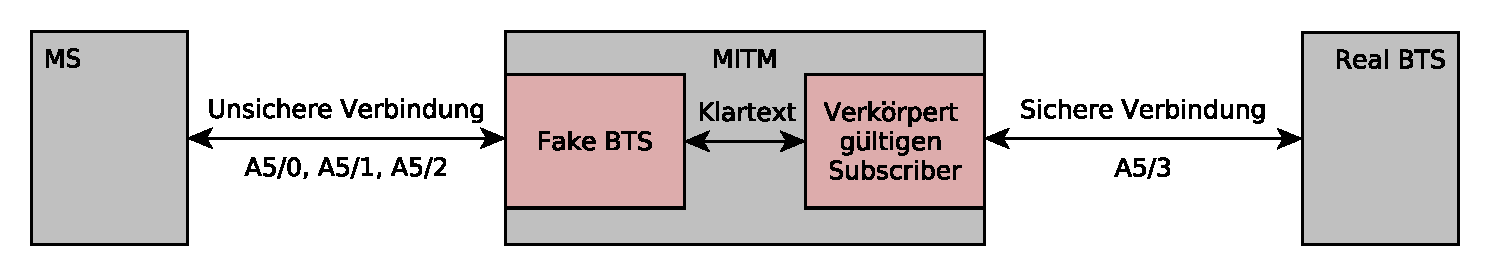
\includegraphics[width=0.9\linewidth]{figures/mitm_air_interface.pdf}
	\caption[MitM in Funkschnittstelle]{\ac{MitM} in der Funkschnittstelle} \label{fig:mitm-air-interface}
\end{figure}

Die Interoperabilität der neuen Standards mit \ac{GSM} stellt ein weiteres Problem dar. So ist es möglich auch in 3G oder 4G Netzen den Fallback auf den \ac{GSM}-Standard zu erzwingen, um dessen Schwachstellen ausnutzen zu können. So gelingt es \citet{meyer2004man} \citet{perez2011practical} den \ac{MitM} Angriff auf 3G Netzwerke auszuweiten.

Eine weitere Schwachstelle ist der fehlende Integritätsschutz der übertragenen Daten. So kann weder die \ac{MS} noch die \ac{BTS} die ungewünschte Manipulation von empfangenen Daten bemerken. Die Nachrichten enthalten Paritätsbits aus Firecode oder \ac{CRC}, \citepauthor{3gpp:05.03}. Beide Verfahren eignen sich wegen ihrer Linearität nicht für den Schutz der Datenintegrität. Daten können so manipuliert werden, dass kein Fehler mehr erkannt wird (siehe \autoref{hdl:einleitung_verschlue_ohne_int}). \todo{cite papers}

\section{Schutz der Identität}

Zum Schutz der Identität der Mobilfunkteilnehmer ist im \ac{GSM} Standard in \citetauthor[2.4]{3gpp:03.03} die Vergabe einer \ac{TMSI} vorgesehen deren zugehörige \ac{IMSI} nur das Netzwerk und das Mobilfunktelefon kennt. Die \ac{MS} identifiziert sich nachdem es vom Netzwerk in einer Location Update Response oder einem \ac{TMSI} Reallocation Request eine \ac{TMSI} zugewiesen bekommen hat nur noch mit dieser beim Netzwerk. Somit ist theoretisch ein Aussenstehender nicht in der Lage herauszufinden, wer gerade auf der Funkschnittstelle kommuniziert, selbst wenn er mithören kann.

Das Netzwerk kann allerdings jederzeit einen Identity Request an die \ac{MS} schicken um deren \ac{IMSI}, \ac{TMSI} oder \ac{IMEI} abzufragen, sollte das Mapping im Netzwerk aus irgendeinem Grund verloren gehen. Da die Verbindung zur \ac{MS} beim Identity Request nicht verschlüsselt sein muss, kann eine Fake \ac{BTS} jederzeit die Identität der Netzteilnehmer herausfinden. Der Begriff des \ac{IMSI}-Catchers taucht bereits in \citet{gobel1996strafprozess} in rechtlichen Zusammenhang auf -- seine Funktionsweise wird ab 1998 z.B. von \citet{piper1998cryptographic} oder \citet{fox2002imsi} mehrfach veröffentlicht.

Da die Standards nicht vorgeben wie oft die \ac{TMSI} neu zugewiesen werden muss, ist die Anonymität der Netzteilnehmer abhängig vom Netzanbieter. Zudem kann eine \ac{MS} für eine Anfrage beim Netzwerk statt seiner zugewiesenen \ac{TMSI} jederzeit auch die \ac{IMSI} verwenden. \todo{Cite sth. + Auswirkungen}

In \ac{GSM} ist auf Daten- und Sprachkanälen optional auch Frequency Hopping, der Wechsel der Trägerfrequenz während der Übertragung, möglich. Die Generierung der verwendeten Sprungsequenzen ist in \citetauthor[Kap. 6.2.3]{3gpp:05.02} spezifiziert. Da Störungen auf einzelnen Frequenzen so nur einen kleinen Teil der Daten betreffen und durch Fehlerkorrekturmechanismen meist korrigiert werden können, wird die Übertragung verbessert.  Die Daten werden zudem vor ungewollten Mithörern geschützt. Ein Dritter, der die Sprungsequenz nicht kennt, kann die empfangenen Daten im Idealfall keiner Verbindung zuordnen. 

In der Realität wird Frequency Hopping oft nicht oder mit deterministische Sprungsequenzen verwendet. Die Identität der Netzteilnehmer ist also nur unzureichend geschützt. \todo{Cite (gsmmap), autnutzung in einem Angriff}

Die Zuordnung der \ac{TMSI} zur \ac{IMSI} ermöglicht auch die lokale Ortung des Teilnehmers durch Messung seines Funksignals. Es gibt zudem auch mehrere Möglichkeiten zur Lokalisierung, die Schwachstellen des im Core-Netzwerk verwendeten \ac{SS7} ausnutzen \citep{Mourad:fall-of-ss7} auf die hier nicht näher eingegangen wird. \todo{Aktiv schreibe: wenn ein angreifer kann, dann\\ zitat für ortung, weitere voraussetzungen um orten zu können}

\section{SIM Karte}
\acused{A3}
\acused{A8}
\acused{Ki}

Die Sicherheitsalgorithmen \ac{A3} (Authentifizierung) und \ac{A8} (Schlüsselgenerierung) liegen, wie der geheime Schlüssel \acs{Ki}, auf der externen \ac{SIM} Karte. Die \ac{SIM} hat Schnittstellen zur \ac{MS} um \ac{A3} und \ac{A8} aufzurufen, der in die Algorithmen eingehende \ac{Ki} ist jedoch gut geschützt und nicht ohne Weiteres auslesbar. Eine Schwachstelle im Authentifizierungsalgorithmus, die von \citet{handschuh1998reducing} publiziert wurde ist, dass bei jeder Authentifizierung Informationen über \ac{Ki} preisgegeben werden. Wenn ein Angreifer physischen Zugriff auf eine \ac{SIM}-Karte hat, kann er aus diesen Informationen \ac{Ki} rekonstruieren. Dazu sind etwa 150,000 Authentifizierungen mit bekanntem Klartext nötig. \todo{konkrete referenz}

Da die verwendeten Algorithmen inzwischen bekannt sind, kann eine SIM Karte somit auch kopiert werden. \todo{konkrete referenz}

\section{Praktische Angriffe auf GSM} \label{hdl:grundlagen_praktische-angriffe-gsm}
\todo{der part kommt raus so wie er ist und geht in related works ein}
\subsection{SS7 Schwachstellen - aktueller Angriff um Konten leerzuräumen}

\subsection{Rogue BTS - MitM auf Air Interface}
Man gibt sich als BTS aus, Subscriber versuchen sich mit diesem zu verbinden wenn das Signal das beste ist. Auf Air Interface, wird immer stärkstes Signal ausgewählt. Anbindung in Core Network durch registrierten Subscriber des Angreifers. Frequency Jamming kann benutzt werden um 3g/4g Frequenzen zu blockieren.
Aushandeln von keine Verschlüsselung auf initiazive des rogue bts möglich.
Keine Integrität auf air interface bei GSM!
Passiv / Semi Passiv: Traffic Sniffing, IMSI Catcher\\
Aktiv: Manipulative Eingriffe. Achtung, Kodierung! 


\subsection{Wiederverwendung von Kc}
Die Wiederverwendung eines Schlüssels für mehrere Dienste ermöglicht es Angreifern sich als ein Netzteilnehmer auszugeben ohne sich als dieser authentifizieren zu müssen, sobald sie dessen aktuell verwendeten \ac{Kc} durch Brechen einer verschlüsselten Verbindung herausgefunden haben.

\subsection{Sniffing}
USRP so abrichten dass er die eingehenden Pakete in einem Frequenzbereich mitschneidet. Komplett Passiv.
Gabs da nicht was von Karsten Nohl mit 4 Nokias?
Problem Frequency Hopping beachten um datenverkehr den subsribern zuordnen zu können.

\subsection{DOS - Frequency Jamming}
Frequenzen zuspammen im lokalen bereich des opfers. Dieser kann sich dann entweder gar nicht mehr oder nur noch auf einer freigelassenen Zoelfreuqnz einloggen.

\subsection{DOS - Abmelden eines Subscribers}
Durch imsi detach message ans netzwerk wird ein subscriber komplett aus netzwerk abgemeldet und kann bis zum erneuten einschalten keine nachrichten / calls mehr empfangen.

\subsection{Missbrauch von FemtoBTS}
Manipulierter FemtoBTS als Rogue BTS, ist DIREKT mit mobilfunkanbieter verbunden, muss nicht wie der fake bts eine verbindung zum netzwerk als subscriber herstellen.

\subsection{Imitieren eines gültigen Teilnehmers - Impersonating a subscriber}
IMEI u.a. Kennungen des Telefons kopieren (Werden wohl im Klartext übers air verschickt, RR estabslishment oder so). Mit diesen und geklauten session keys einen Subscriber imitieren.

\subsection{Angriffe im großen Stil - Regierung Polizei etc.}
\href{https://theintercept.com/surveillance-catalogue/}{https://theintercept.com/surveillance-catalogue/}\\
\href{https://theintercept.com/2016/09/12/long-secret-stingray-manuals-detail-how-police-can-spy-on-phones/}{https://theintercept.com/2016/09/12/long-secret-stingray-manuals-detail-how-police-can-spy-on-phones/}

\subsection{Interoperation zwischen UMTS / GSM Sicherheitsmechanismen}
Beim zusammenspiel von GSM/UMTS Komponenten, wann werden welche Sichehheitsmechanismen eingesetzt?

\section{Vergleich mit dem entwickelten Angriff}
\todo{der part geht in related works ein und soll das generelle alleinstellungsmerkmal im vergleich mit anderen attacken herausarbeiten}
Der in dieser Arbeit entwickelte Angriff soll aufzeigen, dass in GSM die Vertraulichkeit der Daten selbst bei Verwendung von aktuellen und sicheren Verschlüsselungs- und Authentifizierungsverfahren nicht gewährleistet ist. Durch die Manipulation des verschlüsselten Anrufaufbaus auf physikalischer Schicht kann ein \ac{MitM}, mit Zugriff auf die Sprachdaten im Klartext eingebunden werden. Da das Entschlüsseln dabei das Netzwerk übernimmt, ist die Attacke unabhängig vom auf der Funkschnittstelle verwendeten Verschlüsselungsalgorithmus anwendbar. Durch zufälliges Padding in der Call Setup Message könnte die Kommunikation gegen den Angriff geschützt werden, was bis jetzt (Stand 2017) in Deutschland von keinem Mobilfunkanbieter umgesetzt wird.\\ \todo{cite!}

\textbf{Vorteile der neu entwickelten Attacke}
\begin{itemize}
\item Sie umgeht komplett das Verschlüsselungsverfahren. Egal wie stark das Verfahren ist, bei unserem \ac{MitM} Handy kommt immer der unverschlüsselte Datenverkehr an. Muss aber Stromverschlüsselung sein.
\item Solange kein Integrationsschutz im \ac{MOC} und der Call Setup Message eingebaut wird, ist die Attacke immun gegen die Stärke des Verschlüsselungsverfahrens.
\item Das Netzwerk übernimmt für den Angreifer in Echtzeit die Entschlüsselung der Daten.
\item Ein Voraussetzung für den Angriff ist ein \ac{MitM} auf dem UM Interface wie in \citet{meyer2004man} beschrieben.
\item Es braucht nur einen (kleineren) Eingriff in die \ac{MOC} Sequenz, um das Angreifer Handy als \ac{MitM} zu initialisieren. Danach erledigt Entschlüsselung und Verschlüsselung automatisch die Hardware unseres Handys bzw. die Netzinfrastruktur. Man benötigt keinen \ac{MitM} auf dem Air Interface über die gesamte Verbindungsdauer.
\item Sobald die Verbindung steht, kann sich der  Anrufer beliebig im Netzwerk bewegen. Wir sind nicht davon abhängig, dass er mit unserem FakeBTS verbunden bleibt. (Falls Handover von Fake BTS auf regulären BTS und damit ausklinken aus dem Air interface möglich.)
\item Unser \ac{MitM} erhält Daten auf oberster Schicht und verwendet für alle Layer darunter die vorhandene Infrastruktur. Um Handover und andere Vorgänge brauchen wir uns nicht zu kümmern.
\item Aktuelle Attacken nutzen Schwächen in der A5/1 Verschlüsselung aus um diese zu knacken. Das ist aufwändig, und Daten können durch Verwendung einer stärkeren Verschlüsselung geschützt werden. Unser Angriff ist unabhängig vom Verschlüsselungsverfahren.
\item unabhängig vom verwendeten Authentifizierungsverfahren! Klappt auch mit UMTS authentifizierung.
\end{itemize}

\textbf{Nachteile der neu entwickelten Attacke}
\begin{itemize}
\item Auf dem angerufenen Mobiltelefon erscheint als Anrufer die Telefonnummer des Angreiferhandys. Durch Rufnummernunterdrückung kann das Problem eingeschränkt werden. Das selbe Problem haben auch Angriffe, die über einen Fake-BTS laufen, da dieser sich zum Netzwerk hin auch als Mobilfunkteilnehmer ausgibt. \todo{testen}
\item Auf dem anrufenden Mobiltelefon erscheint die falsche Mobilfunknummer, falls dieser die Mobile Call Initiated Message auswertet. In der Regel ist das nicht der Fall. \todo{testen}
\item Da das Telefonat den Umweg über das Angreifer Handy nehmen muss, haben wir eine doppelt so große Latenz.
\item Es wird ein \ac{MitM} auf der physikalischen Schicht der Funkschnittstelle benötigt, der Nachrichten in quasi Echtzeit manipulieren kann.
\end{itemize}